\documentclass[12pt, oneside]{article}
\usepackage[letterpaper, margin=1in]{geometry}
\usepackage[english]{babel}
\usepackage[utf8]{inputenc}
\usepackage{amsmath}
\usepackage{amsfonts}
\usepackage{amssymb}
\usepackage{tikz}
\usepackage{tkz-fct}
%\usepackage{pgfplots}
%\pgfplotsset{width=10cm,compat=1.9}
%\usepackage{pgfplotstable}
\usepackage{venndiagram}

\usepackage{fancyhdr}
\pagestyle{fancy}
\fancyhf{}
%\rhead{Name: \hspace{1.5in} }
\lhead{BECA / Dr. Huson / IB Math SL \qquad Name:\\* 12 June 2019}

\vspace{1cm}

\renewcommand{\headrulewidth}{0pt}

\title{Worksheet and test template}
\author{Chris Huson}
\date{March 2018}

\begin{document}

\subsubsection*{\\* Classwork: Regents problem practice}
You may use a calculator, but for the first three problems you won't need one.

\begin{enumerate}

  \item On the axes below, sketch a possible function $p(x) = (x  -a)(x - b)(x + c)$, where $a$, $b$, and $c$ are positive, $a  >b$, and $p(x)$ has a positive $y$-intercept of $d$. Label all intercepts.
  \begin{center}
      \begin{tikzpicture}[scale=2.54/4]
      \draw[thick,<->] (-7.5,0) -- (7.5,0) node[anchor=north west] {\textbf{x}};
      \draw[thick,<->] (0,-7.5) -- (0,7.5) node[anchor=south east] {\textbf{y}};
      \end{tikzpicture}
  \end{center} %Alg2 Regents Aug2017

  \item What does $\displaystyle \left( \frac{-54x^9}{y^4} \right)^\frac{2}{3}$ equal? %Alg2 Regents Aug2017 multiple choice\\[50pt]

\newpage

  \item Julia deposits \$2000 into a savings account that earns 4\% interest per year. The exponential function that models this savings account
  is $y=2000(1.04)^t$, where $t$ is the time in years. Use the rules of exponents to explain why function that correctly represents the amount of money in her savings account in terms of the \emph{monthly} growth rate is $y=2000(1.0032737)^{12t}$. \vspace{4cm}

  \item Jim is looking to buy a vacation home for \$172,600 near his favorite southern beach. The formula to compute a mortgage payment, $M$, is $\displaystyle M=P \cdot \frac{r(1+r)^N}{(1+r)^N-1}$ where $P$ is the principal amount of the loan, $r$ is the monthly interest rate, and $N$ is the number of monthly payments. Jim’s bank offers a monthly interest rate of 0.305\% for a 15-year mortgage.\\*[5pt]
  With no down payment, determine Jim’s mortgage payment, rounded to the nearest dollar. \vspace{4cm}

  \item What is the quotient when $x^3-13x-12$ is divided by $x - 4$?

\newpage

\item Graph $\displaystyle f(x)= 1.05^{12x} +10$ on the set of axes below.
\begin{center}
    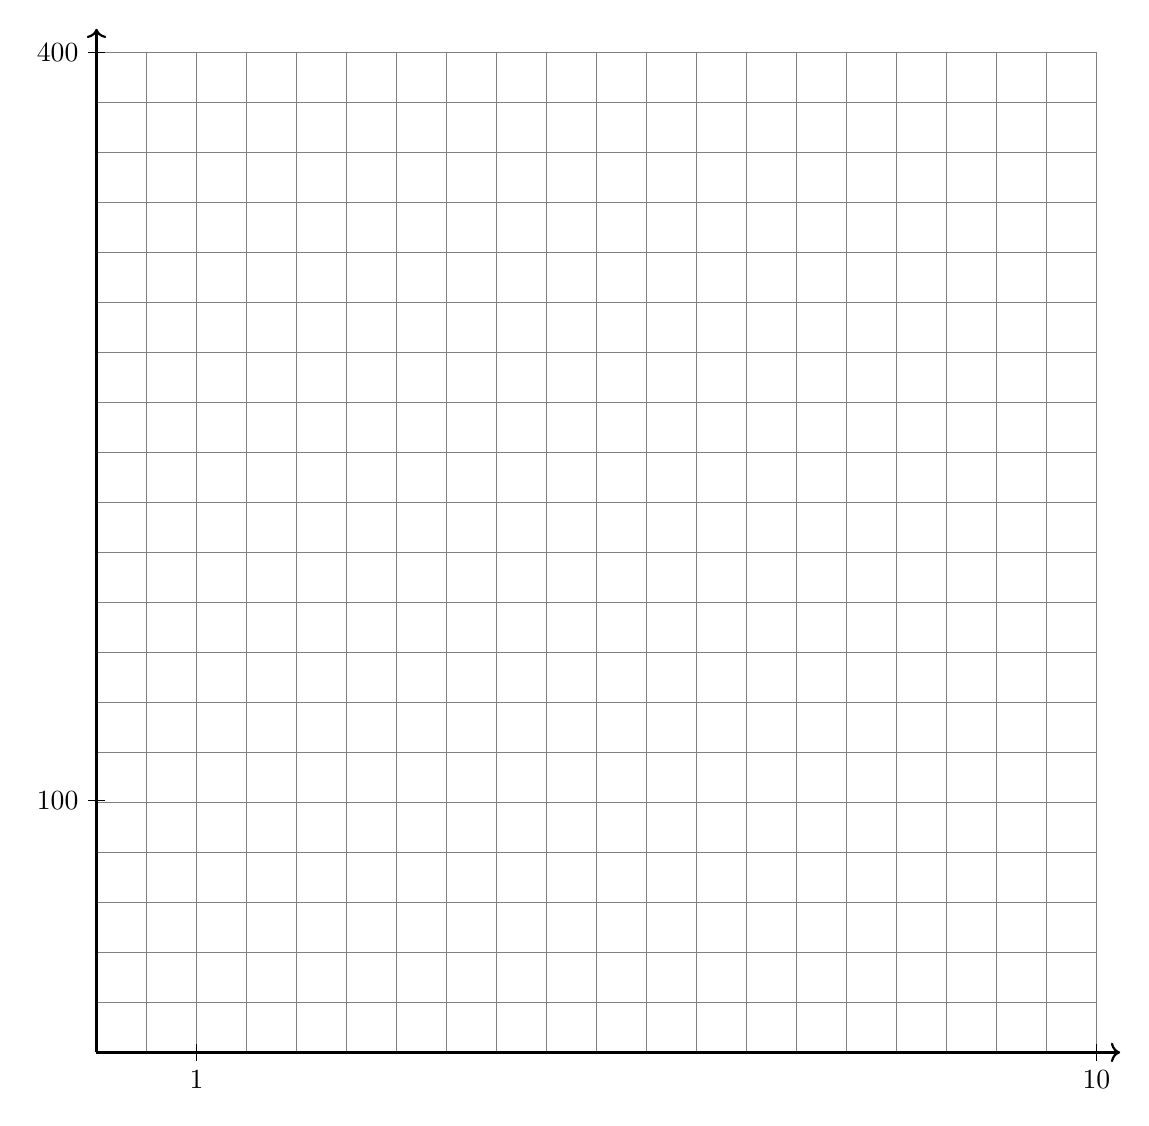
\begin{tikzpicture}
    \draw[step=0.25in,gray,very thin] (0,0) grid (12.7,12.7);
    \draw[thick,->] (0,0) -- (13,0); node[anchor=north west] {x};
    \draw[thick,->] (0,0) -- (0,13); node[anchor=south east] {y};
    \foreach \x in {1.27} \draw (\x cm,3pt) -- (\x cm,-3pt) node[anchor=north] {$1$};
    \foreach \x in {12.7} \draw (\x cm,3pt) -- (\x cm,-3pt) node[anchor=north] {10};
    \foreach \y in {3.2} \draw (3pt,\y cm) -- (-3pt,\y cm) node[anchor=east] {100};
    \foreach \y in {12.7} \draw (3pt,\y cm) -- (-3pt,\y cm) node[anchor=east] {400};
    \end{tikzpicture}
\end{center} %Alg2 Regents Jun2017

\item Use the exponent rules to rewrite the function in \#1, $f(x)$, as exponential function with only $x$ in the exponent. In other words, if $f(x)=b^x+10$, what is $b$?


\end{enumerate}
\end{document}
